\documentclass{article}
\usepackage[UTF8]{ctex}
\usepackage[T1]{fontenc}
\usepackage[utf8]{inputenc}
\usepackage{titlesec}
\usepackage[colorlinks, linkcolor = black]{hyperref}
\usepackage{float}
\usepackage{xcolor}
\usepackage{amsmath}
\usepackage{amssymb}
\usepackage{latexsym}
\usepackage{amsthm}
\usepackage{graphicx}
\usepackage{subcaption}
\usepackage{diagbox}
\renewcommand*\thesubfigure{\roman{subfigure}}
\DeclareMathOperator{\sign}{sign}
\titleformat{\section}[block]{\LARGE\scshape}{\arabic{section}}{1em}{}[]

\title{Homework 8}
\author{PB17000297 罗晏宸}
\date{May 3 2020}

\begin{document}
\maketitle

\section{}
试证明对于不含冲突数据(即特征向量完全相同但标记不同)的训练集,必存在一个与训练集一致(即训练误差为0)的决策树。

\paragraph{解}
\begin{proof}
    决策树中叶节点生成于样本属于同一类或者样本在当前属性集上取值相同时,对于不含冲突数据的训练集,不会出现在当前属性集上取值相同但不同标记的样本,因此决策树的叶节点均为同类样本,即从根节点到每个叶节点的路径都代表一个向量,这个决策树与训练集是一致的。
\end{proof}

\section{}
已知正例点$\boldsymbol{x}_1 = (1, 2)^\mathbf{T}$, $\boldsymbol{x}_2 = (2, 3)^\mathbf{T}$, $\boldsymbol{x}_3 = (3, 3)^\mathbf{T}$,负例点$\boldsymbol{x}_4 = (2, 1)^\mathbf{T}$, $\boldsymbol{x}_5 = (3, 2)^\mathbf{T}$, 试求 Hard Margin SVM 的最大间隔分离超平面和分类决策函数,并在图上画出分离超平面、间隔边界以及支持向量。

\paragraph{解}
在 2 维空间中设 1 维超平面(即直线)方程为$\boldsymbol{\omega} \cdot \boldsymbol{x} - b = (A, B) \cdot (x, y)^\mathbf{T} + C = Ax + By + C = 0$。为避免歧义,用$x_i$与$y_i$表示点$\boldsymbol{x}_1$的分量,也即在二维空间中的坐标。平行的两个间隔边界间距为$\dfrac{\left|C_1 - C_2\right|}{\sqrt{A^2 + B^2}}$,对于数据集求间距的最大值点,即求
\begin{equation*}
    \arg\max
    \left\{
    \begin{aligned}
         & \frac{\left|2B-A\right|}{\sqrt{A^2+B^2}}, & -2 \leqslant           & \frac{A}{B} < -1,            &  & C_1 = -3A - 3B, &  & C_2 = -2A - B  \\
         & \frac{\left|B\right|}{\sqrt{A^2+B^2}},    & -1 \leqslant           & \frac{A}{B}  < -\frac{1}{2}, &  & C_1 = -3A - 3B, &  & C_2 = -3A - 2B \\
         & \frac{\left|2 A\right|}{\sqrt{A^2+B^2}},  & -\frac{1}{2} \leqslant & \frac{A}{B} \leqslant 0,     &  & C_1 = -A - 2B , &  & C_2 = -3A - 2B \\
    \end{aligned}
    \right.
\end{equation*}
得到
\begin{equation*}
    \frac{A}{B} = -\frac{1}{2},\ C_1 = -\frac{3B}{2},\ C_2 = -\frac{B}{2}
\end{equation*}
\begin{figure}
    \centering
    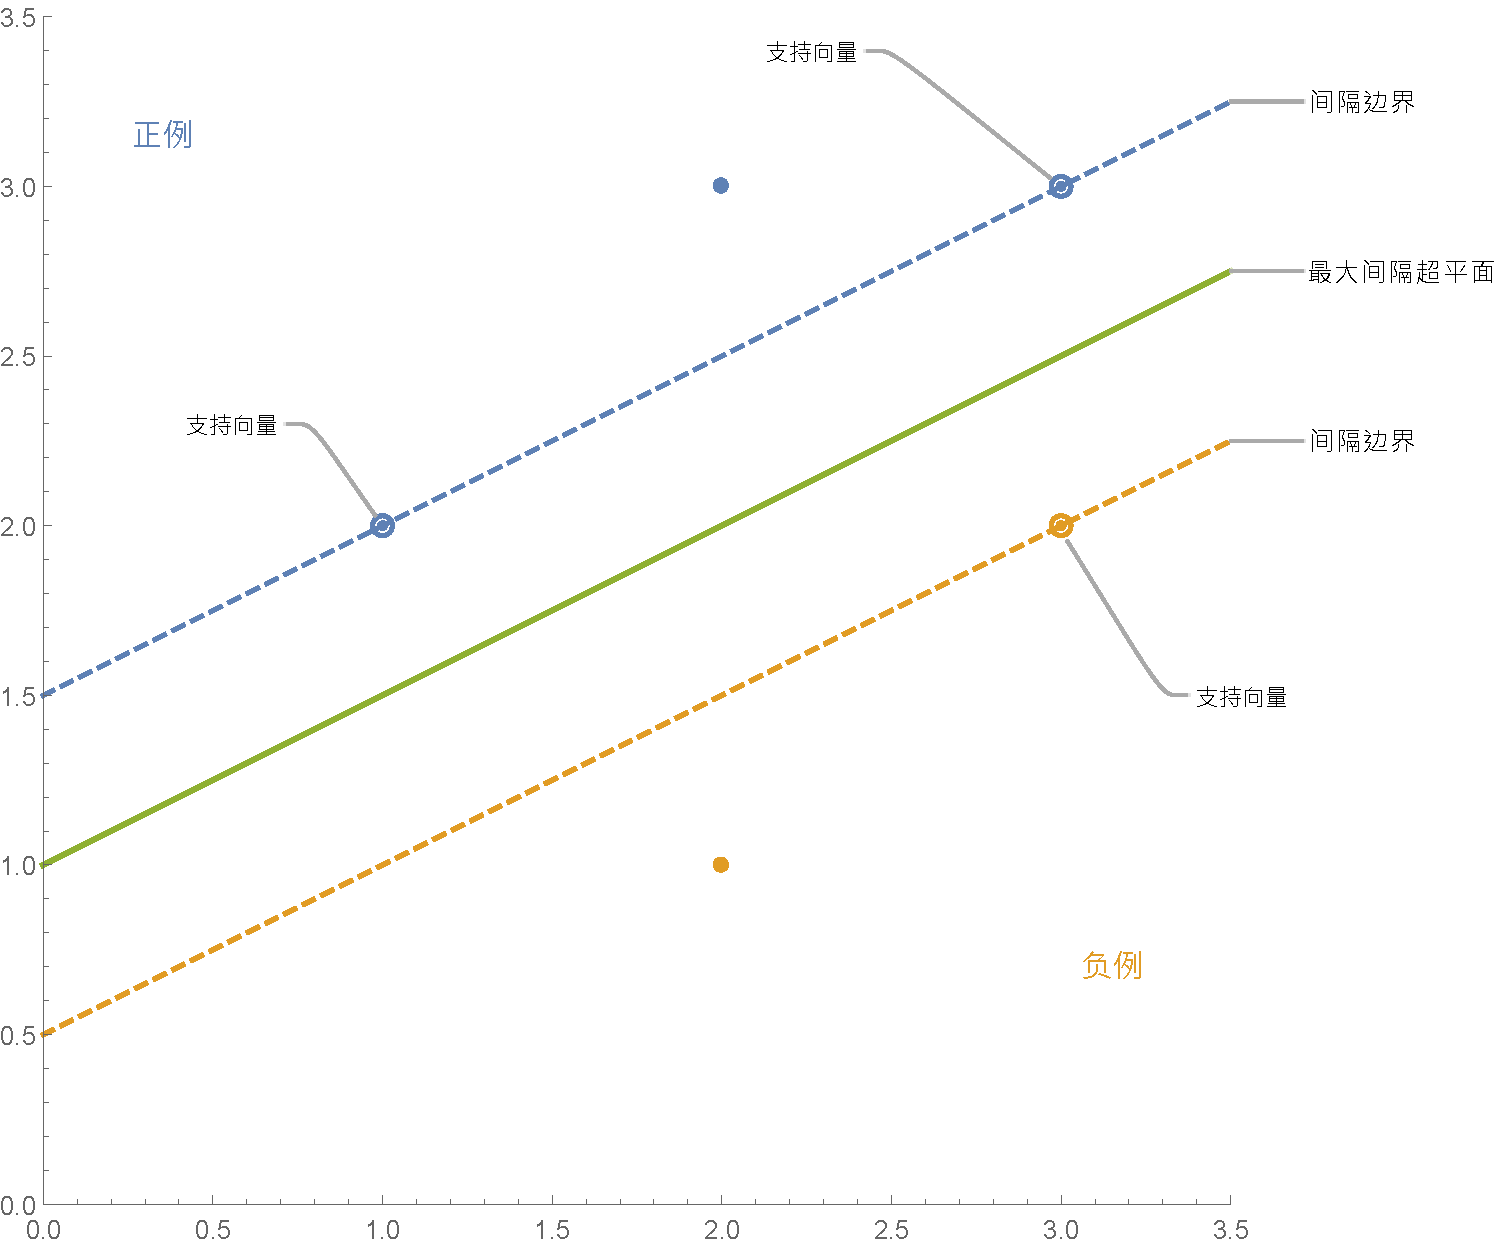
\includegraphics[width = \textwidth]{Figure/SVM.pdf}
    \caption{最大间隔分离器、间隔边界与支持向量}
    \label{SVM}
\end{figure}
如图\ref{SVM}所示,最大间隔分离超平面$\{\boldsymbol{x} : \boldsymbol{\omega} \cdot \boldsymbol{x} - b = 0\}$,其中$\boldsymbol{\omega} = (-1, 2),\ b = 2$,即
\begin{equation*}
    \{\boldsymbol{x} : -x + 2y - 2= 0\}
\end{equation*}
分类决策函数为
\begin{equation*}
    h(x) = \sign{\{\boldsymbol{\omega} \cdot \boldsymbol{x} - b\}} = \sign{\{ -x + 2y - 2\}}
\end{equation*}
\end{document}